\section{Messen von Induktivitäten}
Die Messung von Induktivitätswerten wird nach allen anderen Messungen als separater Teil mit allen
gefundenen Widerständen mit weniger als \(2100\Omega\) durchgeführt.
Das Messverfahren beruht auf dem Prinzip, dass beim Schliessen des Stromkreises der Strom nach
der Formel \(Il~=~Imax~\cdot~(1~-~\exp{\frac{-t}{\tau}})\) ansteigt.
Die Zeitkonstante \(\tau = \frac{L}{R}\) ist proportional zu der Induktivität~\(L\), aber umgekehrt
proportional zum Widerstand~\(R\). 
Der Strom kann hier nur indirekt über den Spannungsabfall an einem Widerstand
gemessen werden.

Leider wird durch den relativ hohen Widerstand \(680\Omega\) die Zeitkonstante zusätzlich verringert, was
wiederum die Messung von kleinen Induktivitäten mit dem Takt von \(8MHz\) zusätzlich erschwert.
Um die Zeitkonstante zu bestimmen, wird die Spannung am \(680\Omega\)-Widerstand als Stromsensor
mit dem analogen Komparator überwacht. Wenn der Spannungsabfall am \(680\Omega\)-Widerstand grösser als
die Vergleichs-Spannung der internen Spannungsreferenz wird, meldet der Komparator dies an den beim
Stromeinschalten gestarteten 16-Bit-Zähler weiter, der daraufhin den Zählerstand dieses
Ereignisses festhält. Eventuelle Überläufe des Zählers werden vom Programm mitgezählt. 
Wenn die Spannung grösser ist, wird der Zähler sofort angehalten und aus dem festgehaltenen Zählerstand und
dem Überlaufzähler die Gesamtzeit bestimmt.
Der Anschluss der Spule wird wieder von VCC auf GND geschaltet, und über eine Spannungsüberwachung beider
Anschlüsse gewartet, bis kein Strom mehr festgestellt wird.
Das Schaltbild~\ref{fig:Inductance} zeigt ein vereinfachtes Diagram der Messsituation.

\begin{figure}[H]
\centering
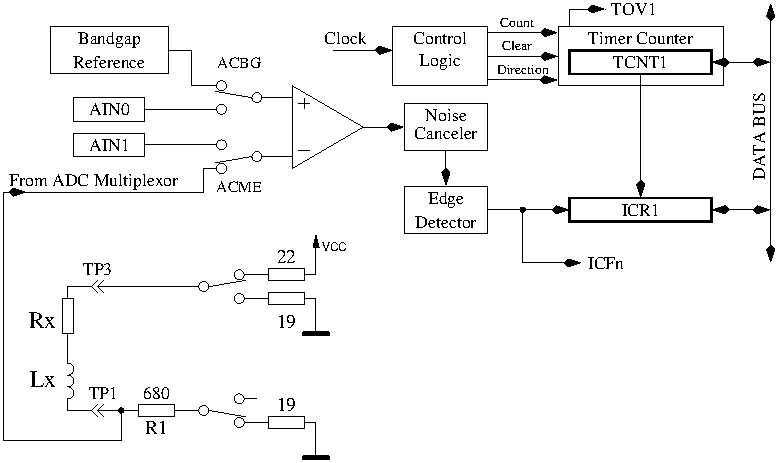
\includegraphics[]{../FIG/Inductance.pdf}
\caption{Messung von Induktivitäten mit dem Komparator}
\label{fig:Inductance}
\end{figure}

Aus der Versorgungsspannung VCC und der Summe aller Widerstände im Stromkreis kann der Maximalstrom Imax und
daraus der Anteil der Vergleichsspannung im Verhältnis zur Maximalspannung am \(680\Omega\)-Widerstand
\(Umax~=~Imax~\cdot~(680~+~19)\) bestimmt werden.
Mit der Formel \(L~=~-\frac{t~\cdot~Rges}{\log{(1~-~\frac{Uref}{Umax})}}\) kann die Induktivität bestimmt werden.
Der natürliche Logarithmus wird im Programm mit einer Tabelle ermittelt.
Die Auflösung der Induktivität wird für diese Art der Messung auf \(0,1mH\) gesetzt.

Um auch kleinere Induktivitäten messen zu können, wird der \(680\Omega\)-Widerstand im Stromkreis weggelassen,
wenn der Widerstandswert der Spule kleiner \(24\Omega\) gemessen wurde. Als Messwiderstand für die Strom-Messung
dient in diesem Fall der Ausgangswiderstand der Ausgabeports (\(19\Omega\)). In diesem Fall wird der Spitzenstrom grösser
als es die Spezifikation des ATmega erlaubt. Da das nur für eine sehr kurze Zeit passiert, erwarte ich keine Schäden.
Um eine längere Zeitdauer mit überhöhtem Strom auszuschliessen, wird die zusätzliche Messung mit 
verzögertem Zählerstart immer mit \(680\Omega\)-Widerstand durchgeführt.
Für diesen Typ der Messung wird die Auflösung der Induktivität auf \(0,01mH\) gesetzt.
Um die Messergebnisse an den tatsächlichen Induktivitätswert anzugleichen, wird vom Zählerstand ein
Nulloffset von 6 abgezogen, wenn ohne \(680\Omega\) gemessen wurde. Sonst wird ein Nulloffset von 7 oder 8 berücksichtigt.


Bei großen Induktivitäten können parasitäre Kapazitäten den Strom so schnell ansteigen lassen, dass
die Spannungsüberwachung mit dem Komparator sofort anspricht. Um dennoch die Induktivität bestimmen zu
können, wird die gleiche Messung noch einmal gemacht, aber der Zähler etwas später gestartet, damit
der Spannungsanstieg durch den Stromzuwachs der Induktivität und nicht die Stromspitze durch die
Steukapazität gemessen wird.
Die Messungen werden in beiden Stromrichtungen durchgeführt.
Von den beiden Messungen in gleicher Stromrichtung wird das höhere Messergebnis verwendet.
Von den Messungen in verschiedenen Stromrichtungen wird der kleinere Wert als Resultat der Induktivitätsmessung genommen.

\subsection{Ergebnisse der Induktivitäts-Messungen}
Die Abbildung~\ref{fig:Induct328p} zeigt die Messergebnisse verschiedener Induktivitäten.
Die Induktivitäten über \(1 H\) sind Relais und Primärwicklungen von Netztrafos, die wegen
der Remanenz des Eisenkerns schwierig zu messen sind.

\begin{figure}[H]
\centering
\includegraphics[width=18cm]{../GNU/induct328pGE.pdf}
\caption{Induktivitäts-Messfehler von 15 verschiedenen ATmega}
\label{fig:Induct328p}
\end{figure}

\subsection{Messung kleiner Induktivitäten mit der Sampling Methode}

Die kleinste erfassbare Induktivität bei der normalen Meßmethode beträgt 0.01~mH.
Für Hochfrequenzanwendungen ist aber die Messung kleinerer Induktivitätswerte sinnvoll.
Die normale Messung verwendet für die Induktivitätsbestimmung den Stromanstieg in der Spule.
Dieser Weg ist für die Sampling Methode nicht verwendbar, da für die Messung keine 
zusätzlichen Widerstände verwendet werden. Der Strom erreicht damit schnell unzulässig hohe
Werte. Ein Schaden des ATmega wird bei der normalen Messung nur dadurch verhindert, daß
der Strom frühzeitig wieder abgeschaltet wird. Für die Sampling-Methode wäre das Abschalten
schwierig durchzuführen und zusätzlich müßte der kritische Vorgang ja oft hintereinander wiederholt werden.
Aus diesem Grunde hat der Funkamateur Pieter-Tjerk (PA3FWM) eine andere Methode für die
Messung benutzt. Mit einem parallel geschaltetem Kondensator wird mit der Induktivität ein
Schwingkreis gebildet. Mit einem kurzen Strompuls wird der Schwingkreis angeregt und mit
der Sampling Methode versucht, die Eigenfrequenz des Schwingkreises zu bestimmen.
Weil für die ADC-Messung ein Ende der Spule auf Massepotential gehalten werden muß,
ergeben sich zwei Schwierigkeiten. Die Spannung der Schwingung geht natürlich auch
in den negativen Bereich. Hier wird die Schwingung durch die interne Schutzdiode
des ATmega auf etwa 0.6V begrenzt. Damit wird auch die positive Spitzenspannung der
Schwingung auf diesen Wert begrenzt. Daneben kann der ADC nur positive Spannungen messen.
Deswegen fehlt jeder negative Teil der Schwingugen. Anstelle der negativen Spannungen
liest der ADC immer eine Null.
Trotzdem ist es Pieter-Tjerk gelungen, die Eigenfrequenz hinreichend genau aus den
gemessenen ADC-Daten zu bestimmen. Aus der Eigenfrequenz des Schwingkreises läßt sich
die Induktivität berechnen, wenn der Kapazitätswert bekannt ist.
Aus diesem Grunde ist die Kalibration um die Messung einer Parallelkapazität für
die Induktivitätsmessung erweitert worden.
Der Kondensator wird mit der Meldung ,,\mbox{\begin{large}1 \electricC 3~10-30nF(L)\end{large}}''
angefordert. Beim unkalibrierten Tester ist ein Wert von \(18nF\) vorbesetzt.
Die Werte für den Parallelkondensator werden relativ hoch gewählt, um die Eigenfrequenz
des Schwingkreises auch bei kleineren Induktivitäten klein zu halten.
Der Kondensator für die Parallelschaltung sollte eine hohe Güte haben (Folien-Typ),
da auch die Güte des Schwingkreises aus der Abnahme der Spannungsamplitude bestimmt wird.
Bei hoher Güte des Kondensators ist im Regelfall die Spule bestimmend für die Güte des
Schwingkreises.


Für die Bedienung ist bis auf die Parallelschaltung des Kondensators keine weitere
Aktion erforderlich. Der Schwingkreis wird dann normalerweise automatisch erkannt.
Falls der Schwingkreis entdeckt wurde, wird hinter der Induktivität der Text
,,if'' und die angenommene Kapazität des Parallelkondensators in Zeile 2 angegeben.
Für diesen Fall wird der Widerstandswert der Spule am Ende der Zeile 1 mit ausgegeben.
Dem Widerstandwert sollte man auf jeden Fall ohne parallel geschalteten Kondensator überprüfen,
da die Widerstandsmessung am Schwingkreis oft nicht funktioniert!
In einer weiteren Zeile wird die gemessene Schwingfrequenz und die Güte Q angegeben.
Wenn kein Schwingkreis festgestellt wurde, wird der Widerstand und die Induktivität
in Zeile 2 ausgegeben. In einer weiteren Zeile wird die Resonanzfrequenz und die
Güte angegeben, wenn trotz fehlendem Parallelkondensator eine Eigenresonanz der Spule
festgestellt wurde.

Für eine Luftspule mit 6 Windungen und einem parallelgeschaltetem 18nF Kondensator
bestimmt die Samplingmethode folgendes Ergebnis:

\begin{verbatim}
260nH if 18.1nF
2306kHz Q=38.7
\end{verbatim}

Der ATmega328 wurde dafür mit 8 MHz betrieben. In etwa das gleiche Ergebnis erzielt auch
ein 25cm langer Kupferdraht, der zu einem großen Kreis gebogen wurde.
Die gemessene Induktivität ist bei dieser Messung etwas zu hoch, da der Kondensator ein
gewickelter Folienkondensator mit Eigeninduktivität war.
In der folgenden Tabelle \ref{tab:littleInductors} sind die Meßergebnisse mit verschiedenen
Spulen dargestellt, die mit einem Tester bei 16 MHz Taktfrequenz ermittelt wurden.

\begin{table}[H]
\begin{center}
\begin{tabular}{| l | c | c | c | c | c |}
\hline
\hspace{1.5cm} Cp= & 6.68nF    & 11.4nF    & 18.2nF    & 20.3nF    & 33.3nF \\
Lp=           &           &           &           &           &        \\ 
\hline
\hline
3 turns, 13mm & 100nH     & 116nH     & 108nH     & 115nH     & 111nH  \\
 (91.4nH) & 6.039MHz  & 4.358MHz  & 3.568Mhz  & 3.282MHz  & 2.619MHz \\
              & Q=29.9    & Q=15.6    & Q=49.8    & Q=12.1    & Q=31.4  \\
\hline
4 turns, 13mm & 141nH     & 161nH     & 151nH     & 152nH     & 153nH  \\
 (144.9nH)     & 5.172MHz  & 3.724MHz  & 3.03Mhz   & 2.86MHz   & 2.226MHz \\
              & Q=44.8    & Q=16.0    & Q=46.2    & Q=14.6    & Q=30.5  \\
\hline
6 turns, 13mm & 217nH     & 232nH     & 223nH     & 224nH     & 227nH  \\
 (212.5nH)    & 4.18MHz   & 3.094MHz  & 2.492Mhz  & 2.343MHz  & 1.832MHz \\
              & Q=30.5    & Q=18.4    & Q=43.0    & Q=15.4    & Q=31.7  \\
\hline
12 turns, 13mm     & 547nH     & 571nH     & 559nH     & 560nH     & 566nH  \\
 (569.5nH)    & 2.632MHz  & 1.973MHz  & 1.573Mhz  & 1.491MHz  & 1.16MHz \\
              & Q=36.9    & Q=26.4    & Q=50.6    & Q=20.8    & Q=39.2  \\
\hline
27 turns, 11mm & \(1.93\mu H\) & \(1.92\mu H\) & \(2.02\mu H\) & \(2.00\mu H\) & \(2.01\mu H\)  \\
(\(1.9\mu H\)) & 1.403MHz  & 1.067MHz  & 828.5khz  & 789.5kHz  & 615.4kHz \\
              & Q=36.5    & Q=33.4    & Q=43.6    & Q=26.6    & Q=34.5  \\
\hline
\(6.3\mu H\)  & \(6.69\mu H\) & \(6.84\mu H\) & \(6.84\mu H\) & \(6.82\mu H\) & \(6.90\mu H\)  \\
\(7.12\mu H\) & 752.9kHz  & 570.2kHz  & 449.9khz  & 428.1kHz  & 332.3kHz \\
              & Q=28.5    & Q=30.5    & Q=32.3    & Q=25.5    & Q=28.3  \\
\hline
\end{tabular}
\end{center}
\caption{Meßergebnisse von einigen kleinen Induktivitäten}
\label{tab:littleInductors}
\end{table}

Die Kondensatoren in dieser Tabelle sind Exemplare mit niedriger Induktivität wie
die WIMA MKS Serie. Die Spule mit 4 Windungen ergibt mit einem gewickelten \(18.2nF\)
Kondensator eine Induktivität von \(196nH\) anstelle der \(151nH\) aus der Tabelle.
Mit Ausnahme der letzen Induktivität handelt es sich um selbstgewickelte Spulen,
deren berechnete Induktivität in Klammern angegeben ist. Die letzte \(6.3\mu H\) Spule
ist ein industriell gefertigtes Exemplar, das mit \(6.3\mu H\) beschriftet ist.
Die Messung mit einem RCL-Meßgerät ergibt bei 100kHz aber eine Induktivität von \(7.12\mu H\)!
In der Tabelle fallen auch die unterschiedlichen Güten bei gleicher Spule und fast gleicher
Parallelkapazität auf. Bei der Spule mit 12 Windungen beträgt die Güte mit dem \(18.2nF\)
Kondensator \(50.2\), bei der Parallelkapazität \(20.3nF\) aber nur \(20.8\).
Das legt den Verdacht eines Programmfehlers nahe.
Zur Kontrolle werden in Bild \ref{fig:W12compare} die Daten des ADC-Wandlers 
für die Spule mit 12 Windungen und den \(18.2nF\) und \(20.3nF\) Kondensatoren gegenübergestellt.
Auch bei den Rohdaten ist der Unterschied für beide Varianten des Schwingkreises deutlich
zu erkennen. Wahrscheinlich ist der verwendete Kondensatortyp die Ursache für den Unterschied
bei der Güte.

\begin{figure}[H]
\centering
\includegraphics[width=16cm]{../GNU/W12compareGE.pdf}
\caption{ADC Daten von zwei Schwingkreisen mit einer 12-Windungen Spule}
\label{fig:W12compare}
\end{figure}

